\section{The project}
\label{sec:project}
The goal of this project is the rapid development of a neural network for low 
power systems, hence the need to resort to a technique known as 
'fine-tuning' for the realization of our neural network.
In general, if our dataset is not drastically different in context from the 
dataset which the pre-trained model is trained on, we should go for 
fine--tuning.
Pre-trained network on a large and diverse dataset like the \emph{ImageNet} 
captures  universal features like curves and edges in its early layers, that are
relevant and useful to most of the classification problems.
Of course, if your data set represents some very specific domain, we should 
then consider training the network from scratch.
One other concern is that if our dataset is small, fine-tuning the pre-trained 
network on a small dataset might lead to over-fitting, especially if the last few 
layers of the network are fully connected layers, as in the case for \emph{VGG} 
network. 
If we have a few thousand raw samples, with the common data augmentation 
strategies implemented (translation, rotation, flipping, etc.), fine-tuning will 
usually get us a better result.
%
\subsection{Fine-tuning Techniques}
\label{subsec:fine-tuning}
Some general guidelines for fine-tuning implementation:
\begin{itemize}
\item The common practice is to truncate the last layer (softmax layer) of the
pre--trained network and replace it with our new \emph{softmax} layer that are
relevant to our own problem. For example, pre-trained network on \emph{ImageNet} 
comes with a \emph{softmax} layer with $1000$ categories.
\end{itemize}
If our task is a classification on $10$ categories, the new \emph{softmax} layer
of the network will be of $10$ categories instead of $1000$ categories.
We then run back propagation on the network to fine-tune the pre--trained 
weights. Make sure cross validation is performed so that the network will be 
able to generalize well.
\begin{itemize}
\item  Use a smaller learning rate to train the network. 
Since we expect the pre--trained weights to be quite good already as compared 
to randomly initialized weights, we do not want to distort them too quickly and 
too much. 
A common practice is to make the initial learning rate $10$ times smaller than 
the one used for scratch training.
\item It is also a common practice to freeze the weights of the first few layers 
of the pre-trained network. 
This is because the first few layers capture universal features like curves and 
edges that are also relevant to our new problem. 
We want to keep those weights intact. Instead, we will get the network to 
focus on learning dataset-specific features in the subsequent layers.
\end{itemize}
%
\section{Fine-tuning in Keras}
\label{sec:finetuningkeras}
%
I have implemented starter scripts for fine-tuning convnets in Keras. 
The scripts are hosted in my remote 
repository\footnote{https://github.com/frank1789/NeuralNetworks} page.
Implementations of VGG16, VGG19, Inception-V3, and ResNet50 are included. 
With that, you can customize the scripts for your own fine-tuning task.
Below is a detailed walk through of how to fine-tune VGG16 and Inception--V3 
models using the scripts.
%
\subsection{Datatset}
\label{subsec:dataset}
Particular attention is needed in the construction of a good training dataset, 
in fact, as seen before in (\ref{subsec:supervised-learnig}), we deal with a 
supervised learning where we know the response of our labels.
A script is provided that can build a dataset divided into folders: training, 
validation and testing; as you can see a figure \ref{fig:datasetstructure}.
A large number of figures per sample that clearly highlights the characteristics 
that you want to study allows a greater rate of success of the training 
preventing the \emph{overfitting}.
On the other hand, a large number of is not always achievable, thus using some 
augmentation techniques, it virtually allows to increase the observability of a 
images, for example, by rotating, distorting and translating it.
The two train and validated folders are essential for the addition of the 
neural network.
Instead, the test folder contains a set of images that the network has never 
seen and so necessary to measure the degree of confidence acquired in the network.
%
\begin{figure}[htb]
\centering
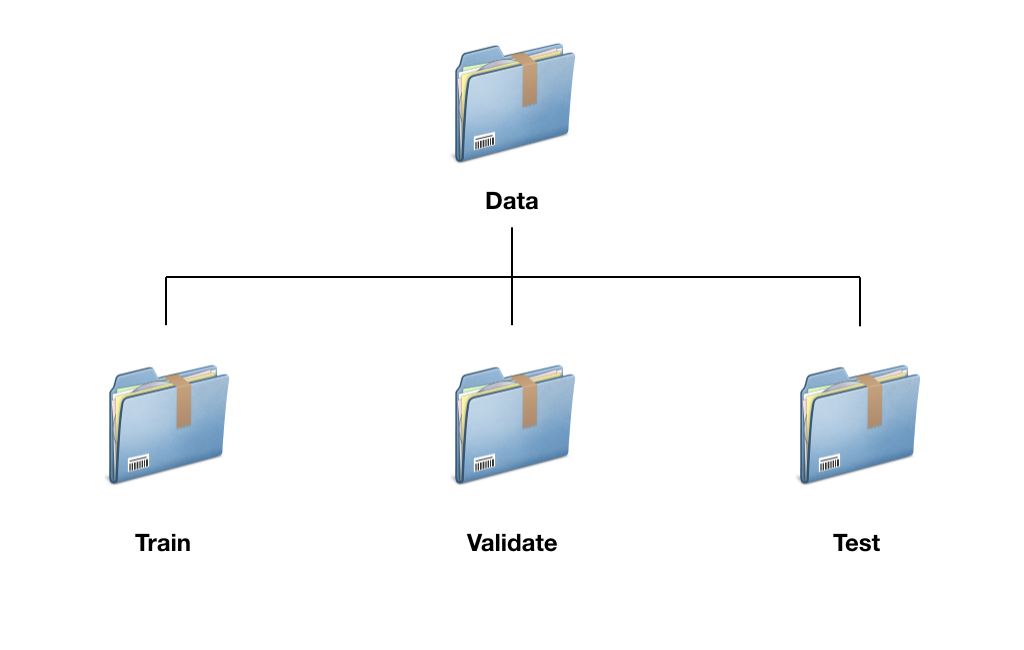
\includegraphics[width=\linewidth]{structure}
\caption{Dataset structure}
\label{fig:datasetstructure}
\end{figure}
%
The choice of using a structure history derives from some methods provided by 
the Keras API, in fact these methods used in the script guarantee greater 
efficiency in the management of the network training process.
In fact, thanks to these it is possible to automatize the processes:
\begin{itemize}
\item crossing the folder structure constituting the dataset;
\item creation of labels within the network;
\item efficient memory management during the training phase;
\item randomness of the set of samples processed;
\item efficient memory management during the validation phase;
\item randomness of the validated sample set;
\end{itemize}
%
\subsection{Fine-tune VGG16} 
\label{subsec:vgg16}
VGG16 is a 16-layer Covnet used by the Visual Geometry Group (VGG) at Oxford 
University in the 2014 ``ILSVRC" (\emph{ImageNet}) competition. 
The model achieves a $7.5\%$ top five error rate on the validation set, which 
is a result that earned them a second place finish in the competition.
%
\begin{figure}[htb]
\centering
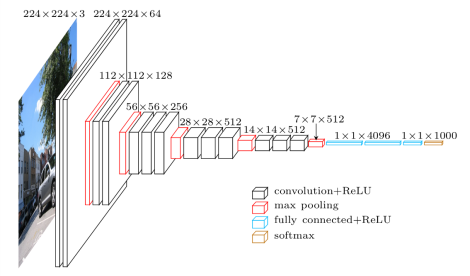
\includegraphics[width=\linewidth]{vgg16}
\caption{Schematic Diagram of VGG16 model}
\label{fig:vgg16schema}
\end{figure}
%
For the first experiment, the network was trained with a dataset from 
the Kaggle\footnote{https://www.kaggle.com} specialist site. 
Withdrawing a binary 
dataset\footnote{https://www.kaggle.com/c/dogs-vs-cats-redux-kernels-edition/data}, 
which consists of only two classes: ``dog" and ``cat".
After using the script, presented in section \ref {subsec:dataset}, the network
is trained, then fine-tuning the model by minimizing the ``\emph{categorical 
cross entropy}" loss function using \emph {stochastic gradient descent} (SGD) 
algorithm.
Notice that we use an initial learning
rate of $0.0001$, which is smaller than the learning rate for training scratch
model usually $0.01$.
It was decided to use this optimization because it has better performance 
during the binary classification.
In fact, after two hundred epochs an accuracy of about $99.96\%$ is reached. 
After it is done, we use the model the make prediction on the validation set 
and return the score for the cross entropy loss, as shown in the 
figure \ref{fig:vgg16resultbin}. \linebreak
\begin{figure}[htb]
\centering
\subfloat[][\emph{Cross entropy accuracy}.]
   {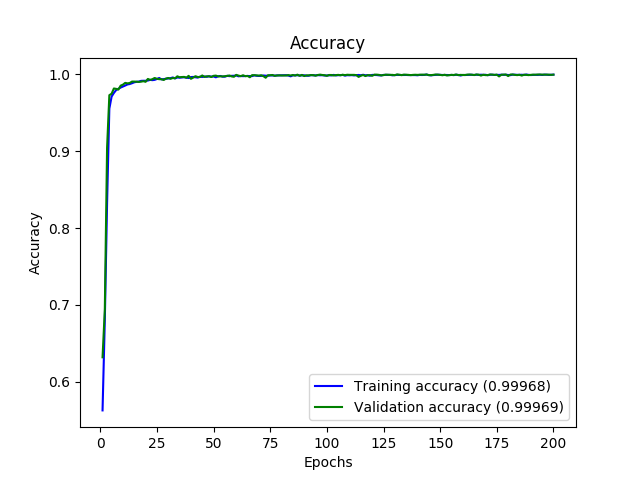
\includegraphics[width=.475\linewidth]{vgg16_catedog_accuracy}} \quad
\subfloat[][\emph{Cross entropy loss}.]
  {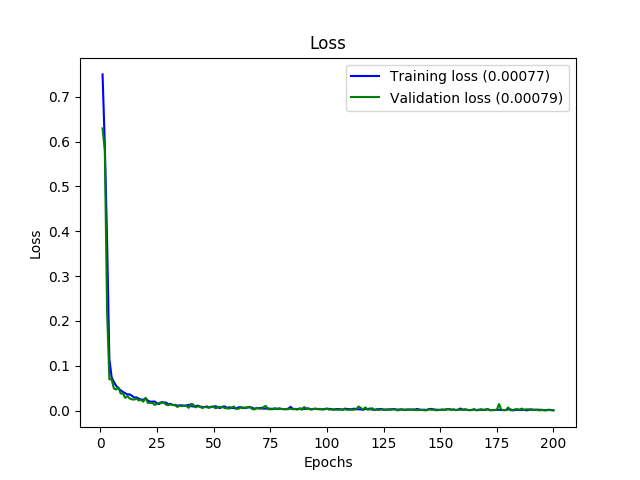
\includegraphics[width=0.475\linewidth]{vgg16_catedog_loss}} 
\caption{VGG16 binary label training result}
\label{fig:vgg16resultbin}
\end{figure}
%
\\The second experiment was instead performed on the 
Simpson\footnote{https://www.kaggle.com/alexattia/the-simpsons-characters-dataset} 
dataset, the famous animated television series, this dataset presents forty-two 
classes, so instead of using an optimization based on SGD it was preferred to 
use an optimizer \emph{Adam} that presents better performance in case of 
multi--label.
In this other case, after two hundred epochs an accuracy of about $99\%$ is 
reached.
Otherwise prediction on the validation set return the score for the cross 
entropy loss, as show in figures \ref{fig:vgg16resultmulti}.
%
\begin{figure}[htb]
\centering
\subfloat[][\emph{Cross entropy accuracy}.]
   {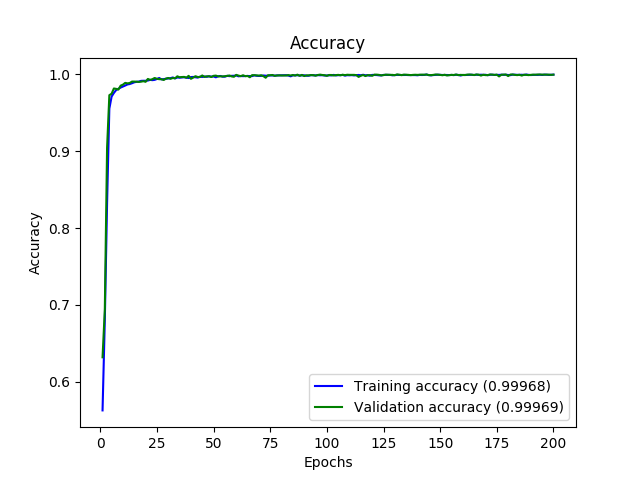
\includegraphics[width=.475\linewidth]{vgg16_catedog_accuracy}} \quad
\subfloat[][\emph{Cross entropy loss}.]
  {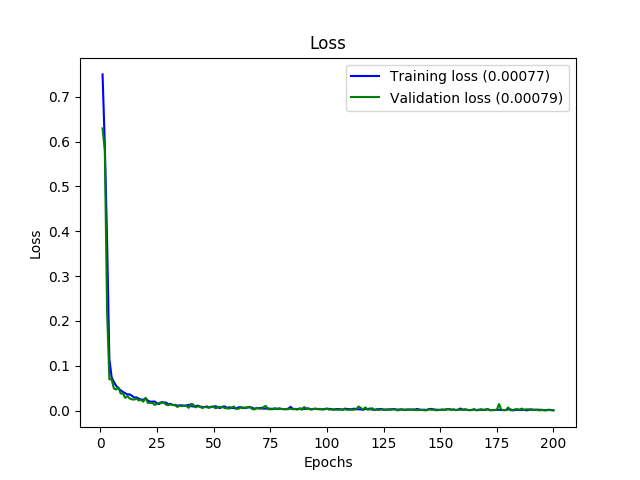
\includegraphics[width=0.475\linewidth]{vgg16_catedog_loss}} 
\caption{VGG16 multi--label training result}
\label{fig:vgg16resultmulti}
\end{figure}
%
\subsection{Fine-tune Inception--V3}
\label{subsec:inception}
Inception--V3 achieved the second place in the $2015$ \emph{ImageNet} 
competition with a $5.6 \%$ top five error rate on the validation set. 
The model is characterized by the usage of the Inception Module, which is a 
concatenation of features maps generated by kernels of varying dimensions.
%
\begin{figure}[htb]
\centering
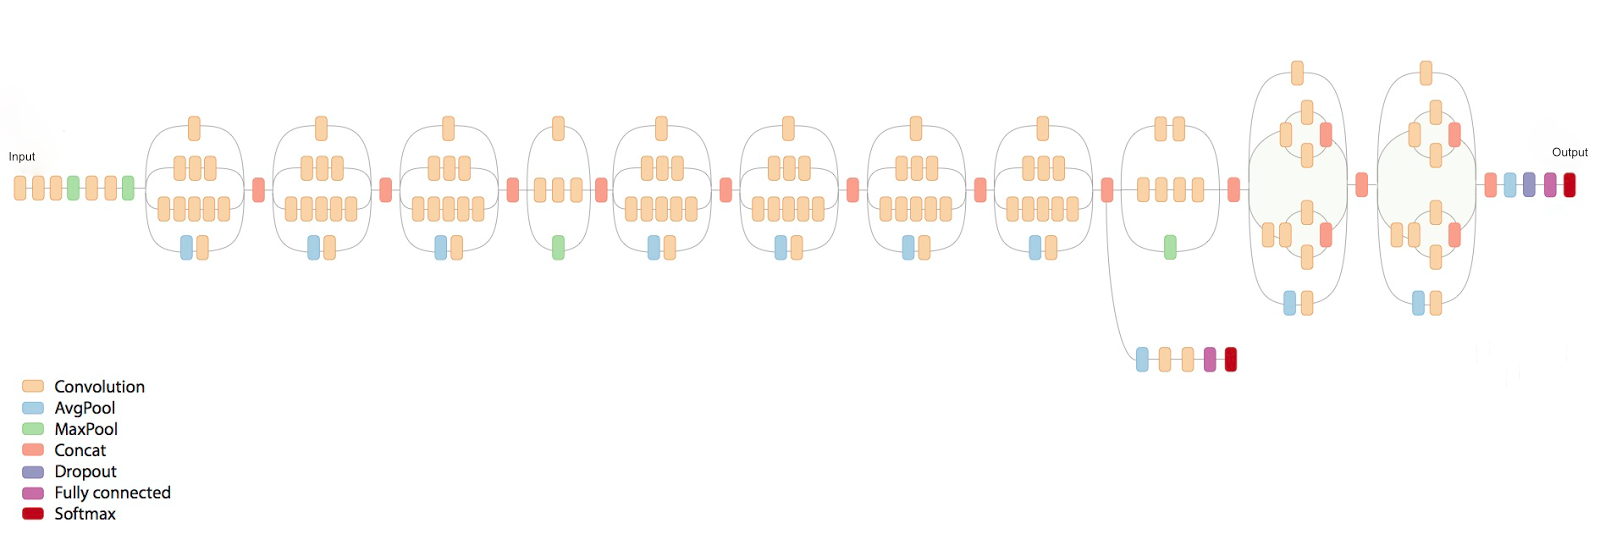
\includegraphics[width=\linewidth]{inception}
\caption{Schematic Diagram of Inception--V3 model}
\label{fig:inceptionV3schema}
\end{figure}
%
As described, for the neural network VGG16 in the section (\ref{subsec:vgg16}), 
the dual experiment was repeated for this neural network.
In this way I obtain, with respect to the previous one, the results shown in figures
for the binary classification.
On the other side the reuses for multi-label classification where an accuracy 
of $99\%$ is observed.
%
\begin{figure}[htb]
\centering
\subfloat[][\emph{Cross entropy accuracy}.]
   {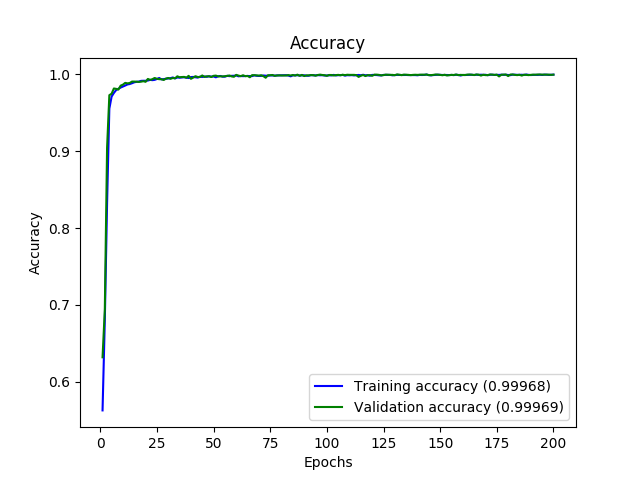
\includegraphics[width=.475\linewidth]{vgg16_catedog_accuracy}} \quad
\subfloat[][\emph{Cross entropy loss}.]
  {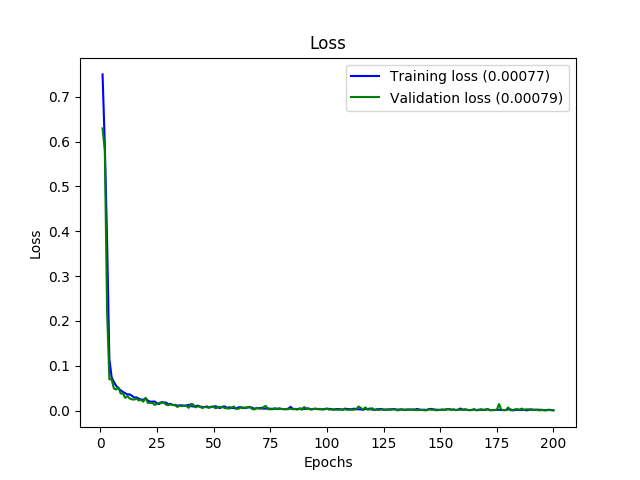
\includegraphics[width=0.475\linewidth]{vgg16_catedog_loss}} 
\caption{Inception binary label training result}
\label{fig:inception-result-bin}
\end{figure}
%
\begin{figure}[htb]
\centering
\subfloat[][\emph{Cross entropy accuracy}.]
   {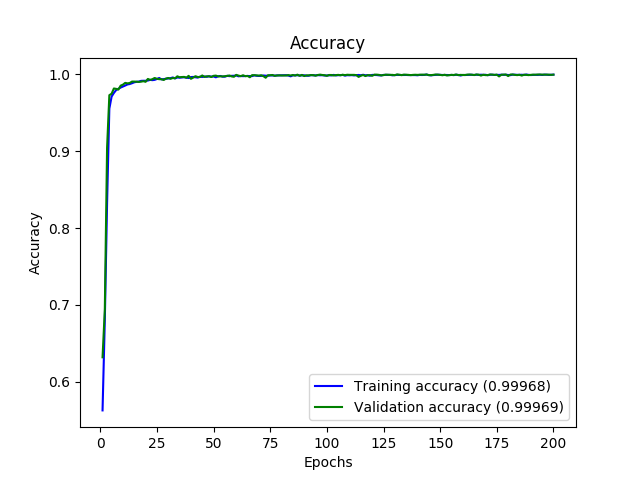
\includegraphics[width=.475\linewidth]{vgg16_catedog_accuracy}} \quad
\subfloat[][\emph{Cross entropy loss}.]
  {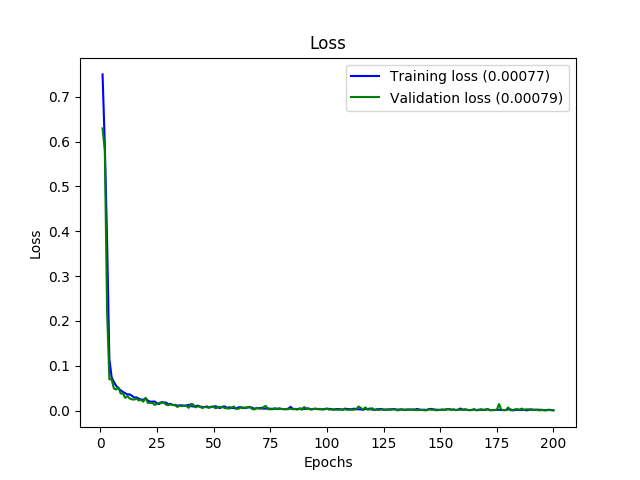
\includegraphics[width=0.475\linewidth]{vgg16_catedog_loss}} 
\caption{Inception multi--label training result}
\label{fig:inception-result-multi}
\end{figure}
%
